% The sharp-front model: the homogenised storage in (z, y) above the fluid in the tube
\documentclass[tikz, border=4pt]{standalone}
% Shared preamble of the PyTES model diagrams: packages, colours and styles.
% Each diagram is a standalone document that inputs this file; build them with build.py.
\usepackage{amsmath}
\usepackage{bm}
\usetikzlibrary{arrows.meta, calc, decorations.pathreplacing, patterns, positioning}

% The PyTES Thermal colour cycle (pytes.plotting.THERMAL) and tints of it
\definecolor{pytesorange}{HTML}{E8590C}
\definecolor{pytesblue}{HTML}{1F4E9C}
\definecolor{pytesteal}{HTML}{14A08A}
\definecolor{pytesamber}{HTML}{F0A930}
\definecolor{pytesplum}{HTML}{A23B72}
\definecolor{pytessky}{HTML}{88C7F0}
\definecolor{pytesink}{HTML}{36312E}

% Materials: the heat transfer fluid, the PCM, the metal (fins and tubes)
\colorlet{fluidfill}{pytessky!75}
\colorlet{pcmfill}{pytesamber!55}
\colorlet{liquidfill}{pytesorange!60}
\colorlet{metalfill}{pytesink!45}
\colorlet{compositefill}{pcmfill!85!metalfill}

\tikzset{
  >={Stealth[length=2.2mm]},
  every picture/.style={line join=round, line cap=round, font=\small},
  outline/.style={draw=pytesink, line width=0.6pt},
  fluid/.style={outline, fill=fluidfill},
  pcm/.style={outline, fill=pcmfill},
  liquid/.style={outline, fill=liquidfill},
  metal/.style={outline, fill=metalfill},
  composite/.style={outline, fill=compositefill},
  flow/.style={->, draw=pytesblue, line width=1.2pt},
  heat/.style={->, draw=pytesorange, line width=1.1pt},
  axis/.style={->, draw=pytesink, line width=0.7pt},
  dimension/.style={<->, >={Stealth[length=1.6mm]}, draw=pytesink, line width=0.5pt},
  guide/.style={draw=pytesink!60, line width=0.4pt, dashed},
  symmetry/.style={draw=pytesink, line width=0.5pt, dash dot},
  label/.style={text=pytesink, font=\small},
  note/.style={text=pytesink, font=\footnotesize, align=center},
}

\begin{document}
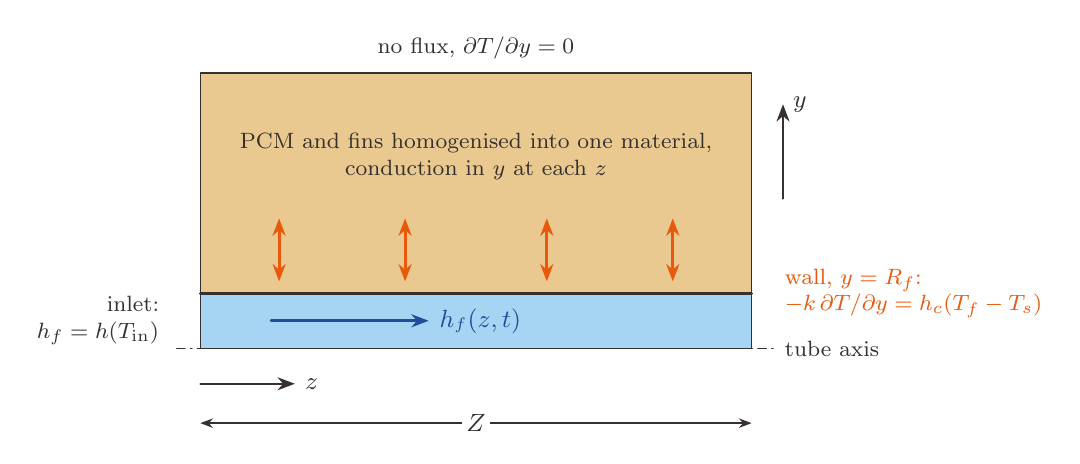
\begin{tikzpicture}
  \def\L{7.0}
  \def\Rf{0.7}
  \def\D{2.8}
  \draw[fluid] (0, 0) rectangle (\L, \Rf);
  \draw[composite] (0, \Rf) rectangle (\L, \Rf + \D);
  \draw[outline, line width=1.1pt] (0, \Rf) -- (\L, \Rf);
  \draw[symmetry] (-0.3, 0) -- (\L + 0.3, 0);
  \node[note, align=center] at (\L/2, \Rf + 0.62*\D)
    {PCM and fins homogenised into one material,\\conduction in $y$ at each $z$};
  % Conduction in y at a few positions along the tube
  \foreach \zc in {1.0, 2.6, 4.4, 6.0} {
    \draw[heat, <->] (\zc, \Rf + 0.15) -- (\zc, \Rf + 0.95);
  }
  \draw[flow] (0.9, \Rf/2) -- (2.9, \Rf/2) node[label, right, text=pytesblue] {$h_f(z, t)$};
  % Boundary conditions
  \node[note, anchor=south] at (\L/2, \Rf + \D + 0.05) {no flux, $\partial T/\partial y = 0$};
  \node[note, anchor=west, align=left, text=pytesorange] at (\L + 0.3, \Rf)
    {wall, $y = R_f$:\\$-k\,\partial T/\partial y = h_c (T_f - T_s)$};
  \node[note, anchor=east, align=right] at (-0.4, \Rf/2)
    {inlet:\\$h_f = h(T_\mathrm{in})$};
  \node[note, anchor=west] at (\L + 0.3, 0) {tube axis};
  % Coordinates
  \draw[axis] (0, -0.45) -- (1.2, -0.45) node[label, right] {$z$};
  \draw[axis] (\L + 0.4, \Rf + 1.2) -- (\L + 0.4, \Rf + 2.4) node[label, right] {$y$};
  \draw[dimension] (0, -0.95) -- (\L, -0.95) node[label, midway, fill=white, inner sep=1.5pt] {$Z$};
\end{tikzpicture}
\end{document}
